\subsection{Acceptances by campaign and geometry}
\label{sec:v505-geometry}
The different mass ranges of the three campaigns partly reflect the boost
of the pair and the active tracker geometry. For an on-axis parent with
energy $E_A=xE_{\rm beam}$, equal sharing gives the small-angle reference
$m\simeq xE_{\rm beam}\theta$, where $2\theta$ is the opening angle.
At $x=1$, a 15 mrad single-track angle corresponds to approximately
15.84, 34.50 and 56.10 MeV in 2015, 2016 and 2021. These scales help explain
the movement of the low-mass turn-on with beam energy. They do not set a
hard mass threshold: azimuth, momentum sharing, magnetic bending and missed
planes all affect whether a pair crosses enough active silicon.

The v5.7.1 study follows prompt $A'\to e^+e^-$ decays through representative
LCDD sensor geometries and the campaign field maps. The daughter momenta
are generated from exact two-body kinematics, rotated into the detector
frame and propagated numerically. A sensor is hit only when the trajectory
crosses its finite active face. Axial and stereo views are counted separately
and then paired within a station when a three-dimensional point is required.
The event displays in Figure~\ref{v571:geometry-figure} use passing trajectories
from this same calculation; they are generated examples, not reconstructed
data events. Transverse distances are expanded to make the sensor faces and
charge-dependent bending visible.

The 2015 and 2016 curves require at least five paired stations per track;
the 2015 positron also requires paired L1 and L2 hits. The 2021 study instead
uses at least ten individual strip-plane hits for the positron and eight for
the electron. This is the explicit v5.7.1 geometry-study specification.
The archived prompt-TC histogram does not establish equivalence to this
hit-count convention, so the geometric curves do not alter the event
selection recorded above.

\begin{figure}[htbp]\centering
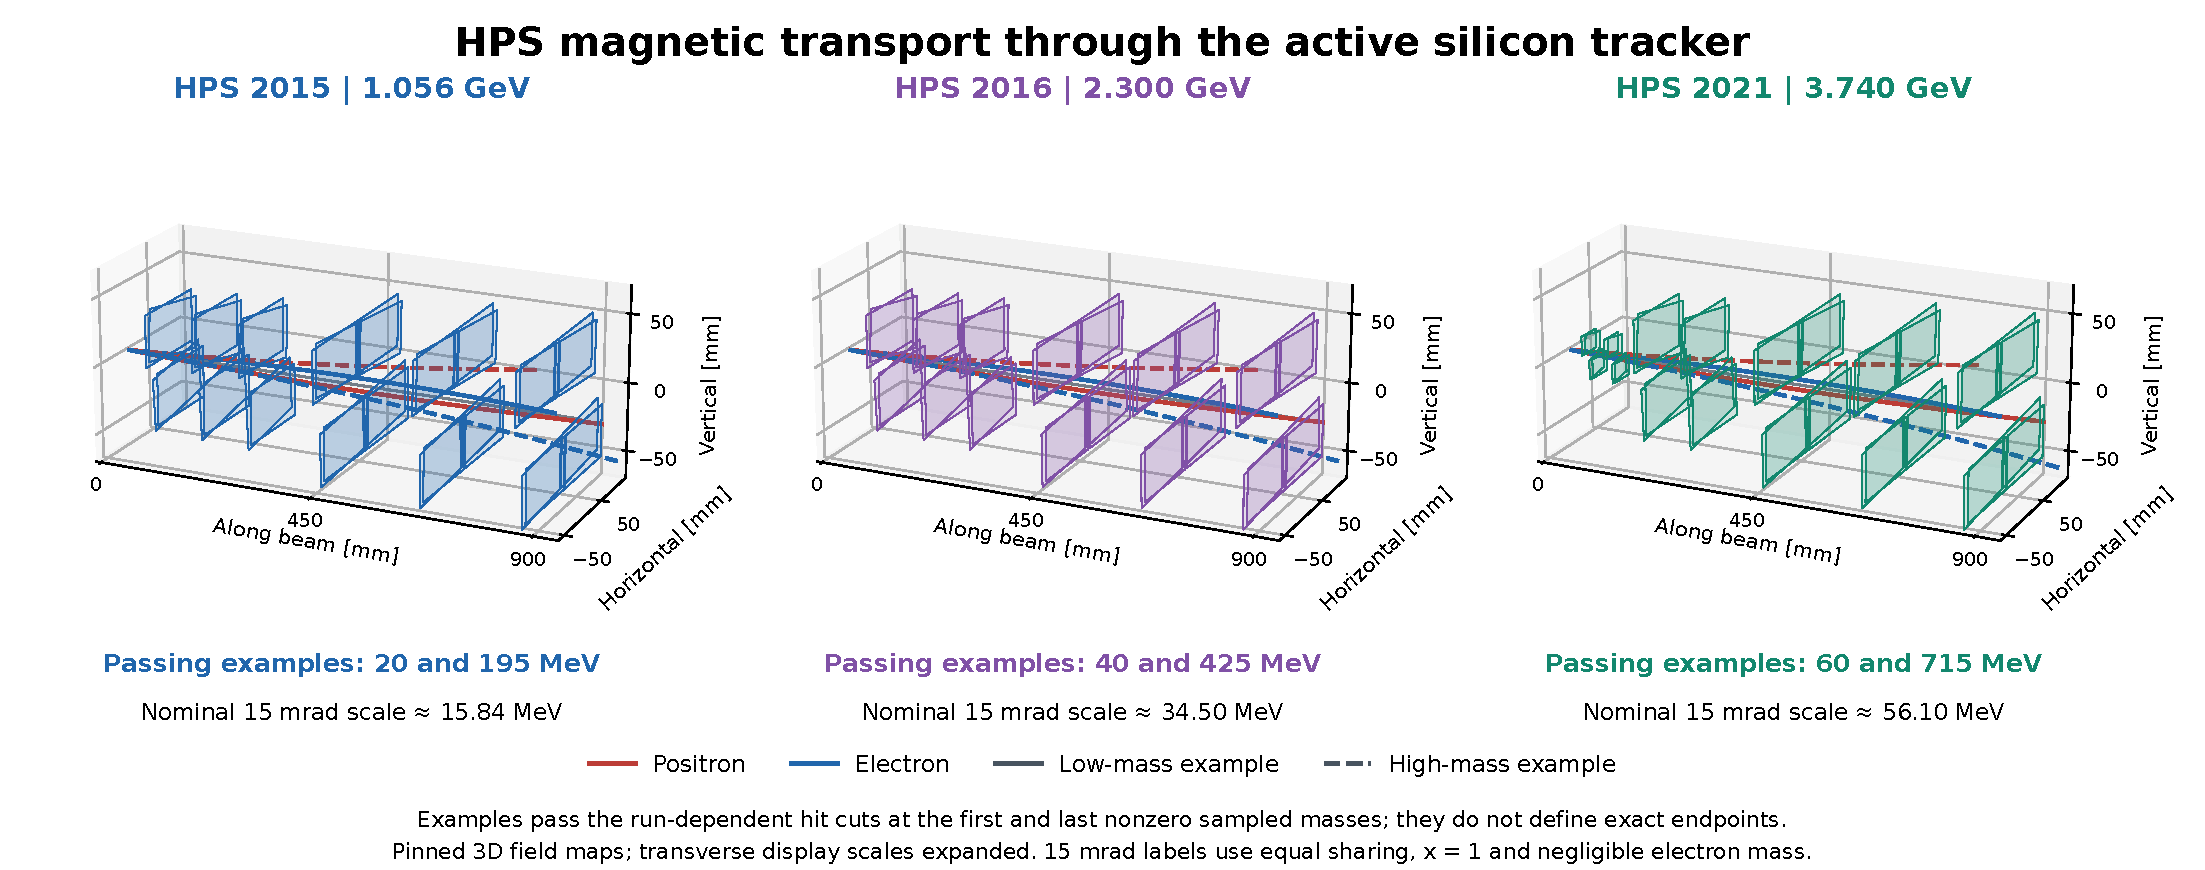
\includegraphics[width=\linewidth]{../figures/HPS_v5p7p1_geometry_illustration.pdf}
\caption{Active sensor geometry and accepted daughter trajectories for the
three campaigns, as shown on slide 5 of the September analysis meeting.
Solid and dashed trajectories illustrate the first and last masses with a
passing orientation on the saved grid. Those examples do not establish
physical acceptance endpoints. Red denotes positrons and blue electrons.}
\label{v571:geometry-figure}\end{figure}

Figure~\ref{v571:overview} averages the hit test over 4096 deterministic decay
orientations per mass, weighted for a transversely polarized vector and
sampled at 5 MeV intervals. At full beam energy, the sampled maxima occur
at 40, 90 and 195 MeV, with accepted fractions of about 26.1\%, 25.9\% and
40.1\%, respectively. Curves at $x=0.8$, with zero field, and with all stations
required separate the effects of boost, bending and the hit requirement.
The larger 2021 fraction also depends on its different sensor layout and
selection; it cannot be attributed to beam energy alone.

\begin{figure}[htbp]\centering
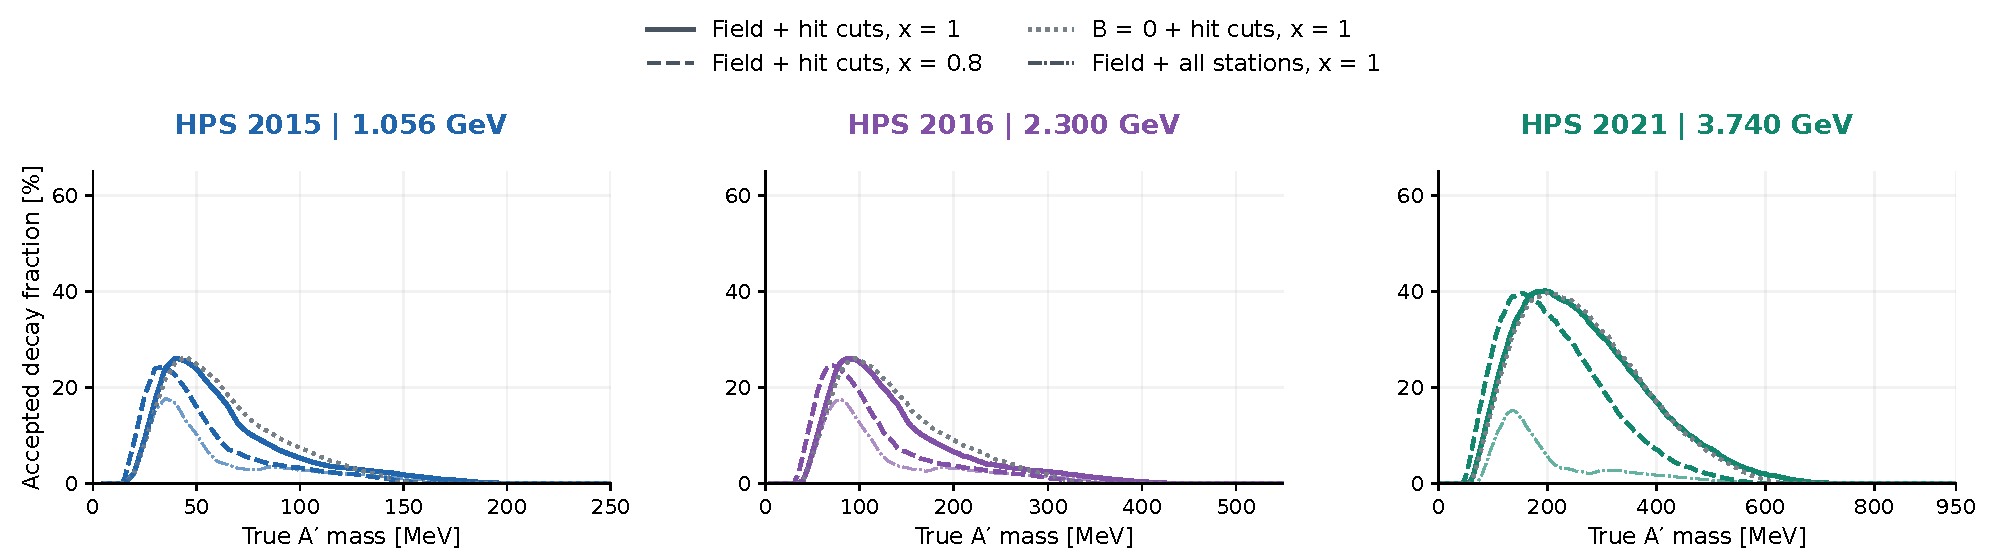
\includegraphics[width=\linewidth]{../figures/v505_campaign_fractions.pdf}
\caption{Conditional geometry-and-field fractions underlying slide 6.
Solid curves use $x=1$ and the campaign hit requirements, dashed curves use
$x=0.8$, dotted curves set the field to zero, and the faint dash--dotted
curves require every station. The parent energy, direction and polarization
are fixed by the stated model. These fractions omit reconstruction, trigger,
material interactions and the remaining analysis cuts.}
\label{v571:overview}\end{figure}

These plots describe which generated daughter trajectories cross the tracker.
A signal efficiency for the resonance search would additionally require the
production energy and angular distributions, material transport, dead channels,
hit finding, trigger and reconstruction, followed by the full event selection.
The geometry calculation therefore supplies no replacement normalization for
the observed limits. Appendix~\ref{app:v505-geometry} documents the geometry,
field units, integration, hit tests and numerical checks in detail.
